%%% License: Creative Commons Attribution Share Alike 4.0 (see https://creativecommons.org/licenses/by-sa/4.0/)
%%% Slides are based heavily on earlier versions of this course taught by Jesper Rudiger.

\documentclass[english,10pt]{beamer}
%\documentclass[english,10pt,handout]{beamer}
%%% License: Creative Commons Attribution Share Alike 4.0 (see https://creativecommons.org/licenses/by-sa/4.0/)
%%% Slides are based heavily on earlier versions of this course taught by Jesper Rudiger and Peter Norman Sorensen.

\DeclareGraphicsExtensions{.eps, .pdf,.png,.jpg,.mps,}
\usetheme{reMedian}
\usepackage{parskip}
\makeatother

\renewcommand{\baselinestretch}{1.1} 

\usepackage{amsmath, amssymb, amsfonts, amsthm}
\usepackage{enumerate}
\usepackage{hyperref}
\usepackage{url}
\usepackage{bbm}
\usepackage{color}

\usepackage{tikz}
\usepackage{tikzscale}
\newcommand*\circled[1]{\tikz[baseline=(char.base)]{
		\node[shape=circle,draw, inner sep=-20pt] (char) {#1};}}
\usetikzlibrary{automata,positioning}
\usetikzlibrary{decorations.pathreplacing}
\usepackage{pgfplots}
\usepgfplotslibrary{fillbetween}
\usepackage{graphicx}

\usepackage{setspace}
%\thinmuskip=1mu
%\medmuskip=1mu 
%\thickmuskip=1mu 


\usecolortheme{default}
\usepackage{verbatim}
\usepackage[normalem]{ulem}

\usepackage{apptools}
\AtAppendix{
	\setbeamertemplate{frame numbering}[none]
}
\usepackage{natbib}




\title{Financial Markets Microstructure \\ Lecture 5}

\subtitle{Trade size and market depth, \\ Determinants of illiquidity\\
	Chapters 4 and 5 of FPR}

\author{Egor Starkov}

\date{K{\o}benhavns Unversitet \\
	Spring 2020}


\begin{document}
	
\AtBeginSection[]{
	\frame<beamer>{
		\frametitle{This lecture:}
		\tableofcontents[currentsection,currentsubsection]
}}

\frame[plain]{\titlepage}

%\section{Revision and problems}

\begin{frame}{What did we do last week?}
	\begin{enumerate}
		\item The spread is not only driven by adverse selection: order costs and inventory risk have an effect as well
		\item However, we would expect the dynamic effect of these three different mechanisms to be different
		\begin{itemize}
			\item Order costs: only short-run effect 
			\item Inventory risk: medium-run effect, but should be zero in the long run
			\item Adverse selection: long-run effect 
		\end{itemize}
	\end{enumerate}
\end{frame}


\begin{frame}{Exercises from last time}
	\begin{itemize}
		\item In Absalon, I have attached an article from the Economist, December 14 2013, on the Volcker rule. Discuss the claim that \emph{``In practice banks will probably respond by making markets for a narrow range of securities that already trade frequently, and thus might reasonably be expected to do so in the future. Meanwhile, the securities that now change hands less frequently are likely to be shunned, making them even harder to trade.''}
		\item Two other Bloomberg articles are on Einar Aas and his exclusion from Nasdaq. Use this case to discuss how inventory costs can stem from regulation.
	\end{itemize}
\end{frame}


\begin{frame}{Today}
	\begin{itemize}
		\item \textbf{Trade size}: Relax assumption that trade size is unitary
		\begin{itemize}
			\item Look at \cite{kyle_continuous_1985} model
			\item Why another model? 
			\begin{itemize}
				\item We want to check whether our previous predictions are `robust' to allowing arbitrary trade sizes
				\item We want to analyze `depth' and `price impact'
			\end{itemize}
		\end{itemize}
		\item \textbf{Empirical estimation}
		\begin{itemize}
			\item Before we looked at how to estimate the spread, but without a theory for what drives it
			\item Thus: talk about estimating drivers of the spread
			\item Furthermore:
			\begin{itemize}
				\item Look at estimating price impact/depth
				\item Look at estimating proportion of informed trading
			\end{itemize}
		\end{itemize}
	\end{itemize}
\end{frame}



\section{Trade Size (Kyle model)}

\begin{frame}{Introduction}
	Previously:
	\begin{itemize}
		\item Adverse selection: uncertain whether trader is speculator or noise
		\item For tractability, traders present one period and traded one unit
	\end{itemize}
	Now:
	\begin{itemize}
		\item Allow traders to make any size order
		\item Dealer/market makers (MM) submit continuous supply curve 
		\item Model looks much like Stoll's from last class. But:
		\begin{itemize}
			\item Stoll: analyze inventory risk (risk averse MM), no adverse selection (no informed trading), price taking MM
			\item Kyle: analyze adverse selection (informed trading), no inventory risk (risk neutral MM), MM not price taker
		\end{itemize}
	\end{itemize}
\end{frame}


\begin{frame}{Preview}
	\begin{itemize}
		\item \structure{Speculator}: has private information
		\begin{itemize}
			\item Trades using a `large' speculative market order
			\item Strategically moderates order size to reduce price impact
			\item `Hides' behind noise traders who submit a random size order
		\end{itemize}
		\item \structure{Market makers/dealers (MM)}
		\begin{itemize}
			\item Risk neutral and competitive (zero profits)
			\item Observes aggregate order flow, but cannot distinguish speculative orders from noise orders
		\end{itemize}
		\item Compare to Glosten\&Milgrom: in Kyle orders are cleared by the MM in \textit{batches} rather than one-by-one
	\end{itemize}
\end{frame}


\begin{frame}{Static model of Kyle (1985)}
\begin{itemize}
	\item \structure{Asset}: Trade in one risky asset with value  $v \sim N(\mu, \sigma^2_v)$
	% if v is binary we are pretty much back to GM
	\item \structure{Speculator}: Observes true value $v$ (perfect information)
	\begin{itemize}
		\item Places market order $x$
		\item If the order clears at price $p$: gain is $x(v-p)$
		\item $p$ is \alert{unobserved}: maximizes expected gain (risk neutral)
	\end{itemize}
	\item \structure{Noise trader}: Has random demand $u \sim N(0, \sigma^2_u)$
	\item \structure{MM}: Submits a supply schedule of $(q,p)$ combinations:
	\begin{itemize}
		\item Observes aggregate flow $q=x+u$, but not $x$ and $u$
		\item Competitive (zero profit): $p = \mathbb{E}[v|q]$
	\end{itemize}
	\item \structure{Assumption}: $u$ and $v$ are jointly normal and independent
	\item \structure{Method}: Postulate linear strategy-- then check that this is equilibrium
\end{itemize}
\end{frame}


\begin{frame}{Linear equilibrium}
\begin{itemize}
	\item Look for equilibrium where speculator strategy is linear: \alert{$x=\beta(v-\mu)$}
	\begin{itemize}
		\item Note: $\beta$ is endogenously determined by the equilibrium
		\item $\beta>0$ measures speculator \textit{aggression}
	\end{itemize}
	\item MM knows the speculator's strategy:
	\begin{itemize}
		\item They observe $q=x+u=\beta(v-\mu)+u$, and want to \alert{estimate $v$}
		\item Intuitively, \alert{$\mathbb{E}[v|q] = \mu + \lambda  q$}, where $\lambda $ is the regression coefficient $\mathbb{C}(v,q)/\mathbb{V}(q)$, and recall that $\mu=\mathbb{E}[v]$. We'll show this in a minute.
	\end{itemize}
	\item Since $p=\mathbb{E}[v|q]$, we can use the conditional expectation to get a price impact equation 
	\[
	p-\mu=\lambda q.
	\]
	As before, $1/\lambda$ is a measure of market depth
\end{itemize}
\end{frame}


\begin{frame}{Aside: Normal information model}
\begin{itemize}
	\item \structure{Result}: $v|q$ is normally distributed, with
	\[
	\mathbb{E}[v|q] = \mu + \frac{\mathbb{C}(v,q)}{\mathbb{V}(q)} q,
	\]
	and variance $1/(1/\sigma^2_v + \beta^2 / \sigma^2_u)$
	\item \structure{Proof}:
	\begin{enumerate}
		\item As $q=\beta(v-\mu) + u$ then 
		\begin{align*}
		q|v & \sim N(\beta(v-\mu), \sigma^2_u), \text{ and} \\
		q    & \sim N(0, \beta^2 \sigma^2_v+\sigma^2_u)
		\end{align*}
		Also, note that $\mathbb{C}(v,q)= \mathbb{C}(v, \beta(v-\mu)+u)=\beta\sigma^2_v$
	\end{enumerate}
\end{itemize}
\end{frame}


\begin{frame}{Aside: Normal information model (2)}
	\begin{enumerate}
		\setcounter{enumi}{1}
		\item Bayes' rule gives conditional density
		\[
		f(v|q) = f(v) \frac{f(q|v)}{f(q)} = \frac{K_1 K_2}{K_3} e^{-\alert{\left[\frac{(q-\beta(v-\mu))^2}{2\sigma^2_u }+\frac{(v-\mu)^2}{2\sigma^2_v}\right]} + \frac{q^2}{2(\beta^2 \sigma^2_v + \sigma^2_u)}}
		\]
		where $K_1, K_2, K_3$ are density normalizing constants
		\item Focus on the terms with \alert{$v$}. Algebra gives
		\begin{align*}
		&\alert{\frac{(q-\beta(v-\mu))^2}{2\sigma^2_u} + \frac{(v-\mu)^2}{2\sigma^2_v} }\\
		= &\frac{\frac{1}{\sigma^2_v}+\frac{\beta^2}{\sigma^2_u}}{2}\left(v-\mu-\frac{\beta \sigma^2_v}{\beta^2 \sigma^2_v + \sigma^2_u}q \right)^2 + k
		\end{align*}
		where the residual term $k$ does not depend on $v$
	\end{enumerate}
\end{frame}


\begin{frame}{Aside: Normal information model (3)}
	\begin{enumerate}
		\setcounter{enumi}{3}
		\item Rewriting, this gives us
		\[
		f(v|q) = K_4 e^{-\frac{\structure{\frac{1}{\sigma^2_v}+\frac{\beta^2}{\sigma^2_u}}}{2} \left(v-\alert{\mu-\frac{\beta \sigma^2_v}{\beta^2 \sigma^2_v + \sigma^2_u}q }\right)^2},
		\]
		where $K_4=\frac{K_1 K_2}{K_3}e^{ \frac{q^2}{2(\beta^2 \sigma^2_v + \sigma^2_u)}-k}$ is again a normalizing constant.
		This is  a normal distribution with $\mathbb{E}[v|q] = \mu + \frac{\mathbb{C}(v,q)}{\mathbb{V}(q)} q=\alert{\mu+\frac{\beta \sigma^2_v}{\beta^2 \sigma^2_v + \sigma^2_u}q}$ and $\mathbb{V}[v|q]=\structure{\frac{1}{\sigma^2_v}+\frac{\beta^2}{\sigma^2_u}}$, as claimed. Hence,
		\[
		\lambda = \frac{\beta \sigma^2_v}{\beta^2 \sigma^2_v + \sigma^2_u}.
		\]
	\end{enumerate}
\end{frame}


\begin{frame}{Analysis continued: speculator's strategy}
	\begin{itemize}
		\item The speculator takes for granted the pricing rule $p=\mu+\lambda q$
		\begin{itemize}
			\item The gain is $x(v-p) = x(v-\mu-\lambda x - \lambda u)$
			\item Expected gain is $x(v-\mu-\lambda x)$ since $\mathbb{E}[u]=0$
			\item Maximize this quadratic function of $x$. First-order condition is
			\[
			v-\mu -2\lambda x=0
			\]
			solved by $x=\beta(v-\mu)$ where $\beta=1/(2\lambda)$
			\item Note analogy to monopoly problem
		\end{itemize}
		\item Comment: speculator expects a positive profit (could abstain). Competitive risk-neutral MM earns zero profits. Noise traders lose.
	\end{itemize}
\end{frame}


\begin{frame}{Kyle's static equilibrium}
	\begin{itemize}
		\item Finally, `match' the coefficients:
		\[
		\frac{1}{2\beta}=\lambda = \frac{\beta \sigma^2_v}{\beta^2 \sigma^2_v + \sigma^2_u}
		\]
		i.e. $\beta^2 \sigma^2_v + \sigma^2_u = 2 \beta^2 \sigma^2_v$ which yields
		\[
		\alert{ \beta = \frac{\sigma_u}{\sigma_v}}\text{ and } \alert{ \lambda = \frac{\sigma_v}{2\sigma_u}}.
		\]
		\item Thus: the strategies are optimal given the prices, and the prices optimal given the strategies $\rightarrow $ \textbf{equilibrium}
		\item Speculator is more \textbf{aggressive} when 
		\begin{enumerate}
			\item The informational advantage $\sigma_v$ is smaller (why?)
			\item There's more noise $\sigma_u$ to hide behind (why?)
		\end{enumerate}
	\end{itemize}
\end{frame}


\begin{frame}{}
	\begin{itemize}
		\item \textbf{Market depth}:
		\[
		\frac{1}{\lambda} = 2\beta = 2 \frac{\sigma_u}{\sigma_v}
		\]
		The market is deeper when there is less insider trading
		\item Insider's a priori (before observing $q$) \textbf{expected gain}:
		\begin{align*}
		\mathbb{E}[x(v-\mu-\lambda x)] 
		& =\mathbb{E}[\beta(v-\mu)\left(v-\mu-\frac{v-\mu}{2}\right)] \\
		&=\beta\frac{ \sigma^2_v}{2}=\frac{\sigma_v \sigma_u}{2}
		\end{align*}
		\item Market maker's posterior (after observing $q$) \textbf{variance} for $v$ is
		\[
		\mathbb{V}(v|q) = \frac{1}{1/\sigma^2_v + \beta^2/\sigma^2_u} = \frac{\sigma^2_v}{2}
		\]
		Exactly half the prior variance: \structure{Insider reveals half his information}
	\end{itemize}
\end{frame}


\begin{frame}{Kyle's model: summary}
	\begin{itemize}
		\item \textbf{Dealer/market maker model}: Competitive, risk-neutral (zero profit) dealer chooses a supply schedule
		\item \textbf{Informed trader}: Risk averse, observes signal about asset value and places market order
		\item \textbf{Market clearing}: \structure{Auction}, dealer observes only total demand (informed + noise), total demand clears
		\item \textbf{Insights}: Market depth is decreasing in insider trading, insider always reveals half his information
		\item \textbf{Advantage}: Allow for unlimited insider trade, trader not price-taker
		\item \textbf{Shortcomings}: Still no resale
	\end{itemize}
\end{frame}


\begin{frame}{Extensions}
	\begin{enumerate}
		\item \textbf{Dynamics}
		\begin{itemize}
			\item In a fully dynamic model, the insider reveals less than half of the information in each period. Why?
			\pause \structure{In order to better benefit from informational advantage}
			\pause
			\item In the limit where trade is continuous over $[0,T]$, then $\mathbb{V}(v|q_0, ..., q_t) \simeq (T-t)\frac{\sigma^2_v}{T}$: variance decreases linearly in time. 
			\pause \structure{Model of how to split a large trade over time}
		\end{itemize}
		\pause
		\item \textbf{More insiders}
		\begin{itemize}
			\item More insiders are more competitive; more aggressive
			\item The market is more liquid and more information revealed
			\item In dynamic model with several insiders: rush to trade on common information from the beginning
		\end{itemize}
	\end{enumerate}
\end{frame}


\begin{frame}{}
	\begin{enumerate}
		\setcounter{enumi}{2}
		\item \textbf{Imperfect market maker competition} (Cournot style)
		\begin{itemize}
			\item Finite number of market makers, $k=1,..., K$
			\item Market maker $k$ supplies $y^k=\phi(p-\mu)$
			\item Market clears at price $p$ with $\sum y^k = q$
			\item Strategic market maker takes into account effect of orders on profits
			\item Now: $p=\mu+\lambda q$ where $\lambda = \alpha (K-1)/(K-2) > \alpha$. Why? 
			\pause \structure{Dealers make profit by increasing price sensitivity}
		\end{itemize}
		\pause
		\item \textbf{Risk averse market makers}
		\begin{itemize}
			\item Similar to Stoll (1978) from last time: one trading round
			\item For simplicity no asymmetric information!
			\item Allows for imperfect competition: depth is a factor of $(K-1)/(K-2)$ of what we found for Stoll
		\end{itemize}
	\end{enumerate}
\end{frame}



\section{Determinants of Illiquidity}

\begin{frame}{Introduction}
	\begin{itemize}
		\item What determines illiquidity?
		\begin{itemize}
			\item Chapter 2 discussed empirical measures of illiquidity
			\item Chapters 3 and 4 developed some theories
			\item Can we detect the relative importance of theoretical effects on the measures?
		\end{itemize}
		\item The end of chapter 3 discussed the various price impacts of transaction costs, informed trading, market maker risk aversion (figure 3.9)
		\begin{itemize}
			\item Chapter 4: greater price change when transaction is larger
		\end{itemize}
	\end{itemize}
\end{frame}


\begin{frame}{}
	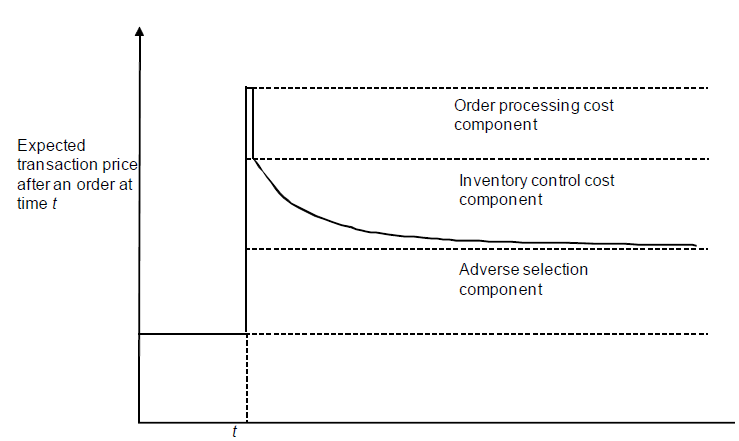
\includegraphics[width=0.8\linewidth]{pics/PriceDiscovery_Image}
\end{frame}


\begin{frame}[label=theory]{Measured price impact and the theories}
	\begin{itemize}
		\item Parameters of interest:
		\begin{itemize}
			\item $\gamma$: order-processing cost
			\item $\lambda$: price impact related to information
			\item $\beta$: price impact related to MM risk aversion
		\end{itemize}
		\item Data:
		\begin{itemize}
			\item Transaction prices $p_t$, net market order flow $q_t$, order sign $d_t$
		\end{itemize}
	\end{itemize}
	\hyperlink{example}{\beamerbutton{Example}}
\end{frame}


\begin{frame}[label=base]{Base model}
	\begin{itemize}
		\item \cite{glosten_estimating_1988} propose
		\begin{equation} \tag{5.7}
		\Delta p_t = \gamma_0 \Delta d_t+ \gamma_1 \Delta q_t + \lambda_0 d_t + \lambda_1 q_t + \epsilon_t%
		\end{equation}%
		Accumulated order flow affects price level via $\lambda$, cyclical order flow gives $\gamma$ in the style of Roll's measure (2.15)
		\begin{itemize}
			\item On NYSE data from early 80s, they find $\gamma_1=\lambda_0=0$ and estimate $\gamma_0=.0465$, $\lambda_1=.0102$
		\end{itemize}
		\item But in the short run, the effect of MM risk aversion would be similar
		\begin{equation} \tag{5.14}
		\Delta p_t = \gamma \Delta d_t + (\lambda + \beta) q_t + \epsilon_t
		\end{equation}
		\begin{itemize}
			\item Then $\lambda$ and $\beta$ are not separately identified. \hyperlink{example2}{\beamerbutton{Example}}
		\end{itemize}
	\end{itemize}
\end{frame}


\begin{frame}[label=extending]{Extending time horizon}
	\begin{itemize}
		\item Figure 3.9: look at price impact over longer periods
		\begin{itemize}
			\item \textbf{\cite{hasbrouck_trades_1988}}: order flow is auto-correlated, so part of the order is not `news' but only moves inventory
			\item \textbf{\cite{huang_components_1997}}: suggest
			\begin{equation}\tag{5.17}
			q_t = \phi q_{t-1} + \eta_t
			\end{equation}
			\item Then (5.14) is modified to \hyperlink{derivation}{\beamerbutton{Derivation}}
			\begin{equation} \tag{5.21}
			\Delta p_t = \gamma \Delta d_t + (\lambda+\beta)q_t - \lambda \phi q_{t-1} + \epsilon_t
			\end{equation}
			\item They estimate the model for 20 major NYSE stocks: $\phi = -.74$ and $ \lambda : \beta :\gamma = 9.59 : 28.65 : 61.76$ percent
			\item Also: larger transactions, greater $\beta$  \hyperlink{example3}{\beamerbutton{Example}}
		\end{itemize}
	\end{itemize}
\end{frame}


\begin{frame}{Extending time horizon (2)}
	\begin{itemize}
		\item Continued...
		\begin{itemize}
			\item \citet*{madhavan_why_1997} find that $\lambda$ is higher in the morning, and $\gamma$ higher in the afternoon
			\item \cite{lyons_tests_1995} had data on a FOREX dealer's inventory, and found $\beta$ very large -- more on this in the course on International Finance
			%TODO: check course references
		\end{itemize}
		%TODO: not 100% sure this is the right Hasbrouck-91, check
		\item Different dynamic approach: \cite{hasbrouck_measuring_1991} uses the long-run impact of an order $q_{t+1}$ on prices $p_{t+T}-p_t$ to identify the informational part of the trade
		\begin{itemize}
			\item The `impulse response' of prices to orders
			\item Opens door to richer time series analysis of transactions data
			\item Our course on Financial Econometrics
		\end{itemize}
	\end{itemize}
\end{frame}


\begin{frame}{Informed trading}
	\begin{itemize}
		\item \citet*{easley_liquidity_1996}: use GM type model to estimate the prob. of informed trading
		\item Traders of a particular type arrive as Poisson process over time, with intensity $\epsilon$
		\begin{itemize}
			\item Probability of observing $n$ traders of a particular type over the trading day is
			\[
			e^{-\epsilon} \frac{\epsilon^n}{n!}
			\]
			\item With probability $\alpha$ there is some information
			\item When there is information, conditional probability $\theta$ that this shows asset value to be high
			\item When there is information, informed traders arrive with intensity $\epsilon_i$; trade as suggested by information
		\end{itemize}
	\end{itemize}
\end{frame}


\begin{frame}{}
	\begin{itemize}
		\item Noise trading
		\begin{itemize}
			\item On all days: uninformed buyers arrive with intensity $\epsilon_b$
			\item On all days: uninformed sellers arrive with intensity $\epsilon_s$
		\end{itemize}
		\item Data for the number of buys and sells allow for estimation of these parameters with \structure{maximum likelihood}
		\begin{itemize}
			\item \citet*{easley_is_2002} estimate the `probability of informed trading' associated with any given order
			\begin{equation} \tag{5.27}
			PIN = \frac{\alpha \epsilon_i}{\epsilon_b + \epsilon_s + \alpha \epsilon_i}
			\end{equation}
			\item With NYSE data from 1983 to 1998 they estimate a median PIN of 19\%, greater for small-cap stocks
			\item PIN is positively correlated with  spread and price volatility
			\item \citet*{grammig_knowing_2001} suggest that PIN is higher when markets are more anonymous
		\end{itemize}
	\end{itemize}
\end{frame}


\begin{frame}{Conclusion}
	\begin{itemize}
		\item Kyle model helps us analyze market depth: i.e. it tells us something about how adverse selection causes spread to vary with trade size
		\item The model has batch clearing instead of the single-unit market of GM
		\item Using the insights from last lecture we can estimate the importance of different components of the spread
		\item Perhaps surprisingly, order costs are by far the largest cost (but estimated on major stocks)
		\item Easley et al.: around 19\% of trading is informed
	\end{itemize}
\end{frame}


\begin{frame}{Exercise}
\begin{itemize}
	\item I uploaded two articles from the Economist, March 7, 2014, both on potential manipulation of prices
	\item Consider these two issues:
	\begin{itemize}
		\item What motivates a trader to manipulate an asset's price? 
		\item Is manipulation easier in a very liquid or a very illiquid market?
	\end{itemize}
\end{itemize}
\end{frame}


\begin{frame}{Next week}
\begin{itemize}
	\item Analyze limit order markets: what is the difference to what we have done so far?
	\item Talk about the role of the `ticks', the priority rule, the interaction between dealers and LOBs, and a way to interpret limit orders
\end{itemize}
\end{frame}




\appendix
\begin{frame}[allowframebreaks]{References}
\bibliography{../teaching}
\bibliographystyle{abbrvnat}
\end{frame}


\begin{frame}<handout:0>[label=example, noframenumbering]
\frametitle{Example}
Data from \cite{lyons_tests_1995}. Deutsche mark trading for one week for one dealer in 1992
\center
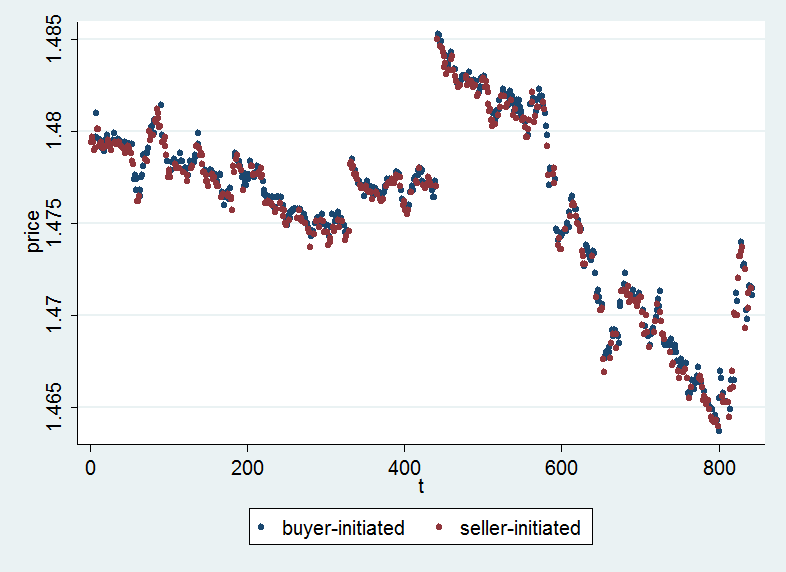
\includegraphics[scale=0.3]{pics/trading}
\end{frame}


\begin{frame}<handout:0>[noframenumbering]
We have inventory data for this particular dealer
\center
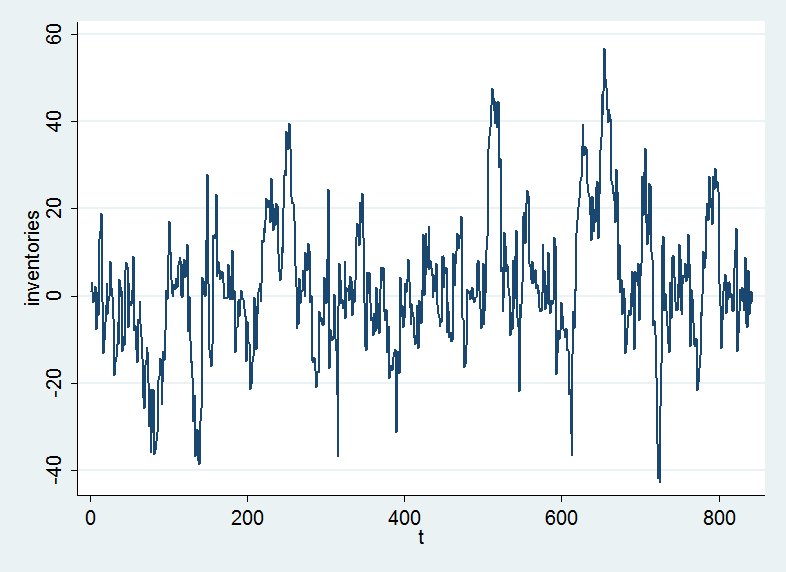
\includegraphics[scale=0.3]{pics/inventory}
\hyperlink{theory}{\beamerbutton{Back}}
\end{frame}


\begin{frame}<handout:0>[label=example2, noframenumbering]
\frametitle{Example}
Estimating equation (5.7) by OLS for our data ($q$ is in million USD)
\quad
\begin{center}
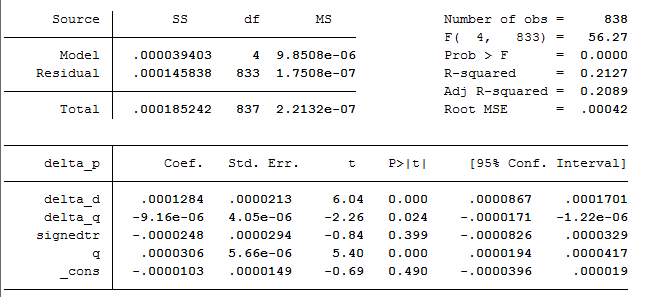
\includegraphics[scale=0.5]{pics/eq57}
\end{center}
We get almost the same restriction.
\end{frame}


\begin{frame}<handout:0>[noframenumbering]
Estimating (5.14) we get
\quad
\begin{center}
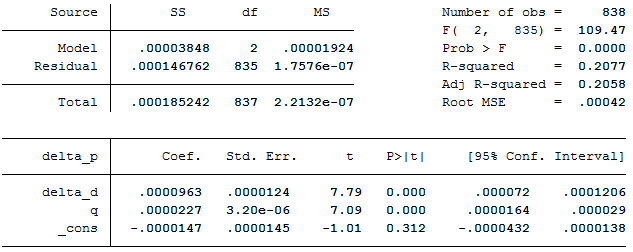
\includegraphics[scale=0.5]{pics/eq514}
\end{center}
\hyperlink{base}{\beamerbutton{Back}}
\end{frame}


\begin{frame}<handout:0>[label=example3, noframenumbering]
\frametitle{Example}
Estimating equations (5.17) and (5.21) `quick and dirty' with GMM, we get
\begin{center}
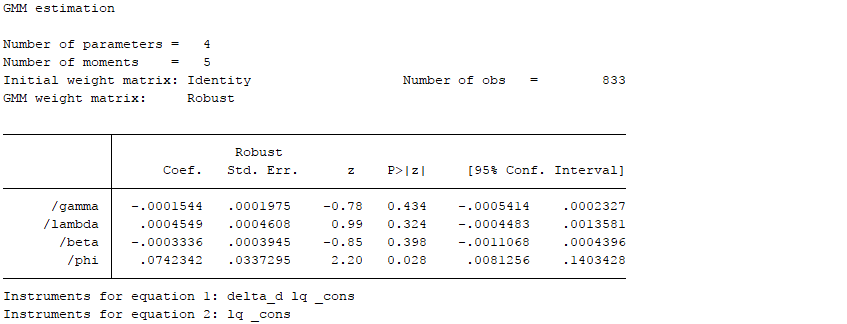
\includegraphics[scale=0.42]{pics/eqgmm}
\end{center}
Unfortunately, these results do not make much sense. We have $\gamma<0$ and $\beta<0$. But both $\beta$, $\gamma$ and $\lambda$ are insignificant.
 \hyperlink{extending}{\beamerbutton{Back}}
\end{frame}


\begin{frame}<handout:0>[label=derivation, noframenumbering]
\frametitle{Derivation of (5.21)}
Suppose $q_t=\phi q_{t-1}+\eta_{t}$. 
\begin{itemize}
\item \textbf{Adverse selection.} Notice that value equation is now
\[
\mu_t=\mu_{t-1}+\lambda[q_t-\mathbb{E}[q_t|\Omega_{t-1}]+\epsilon_t.
\]
Only non-expected part of order flow carries information. 
\item \textbf{Price.} The price equation then becomes
\[
p_t=m_t+\beta q_t+\lambda[q_t-\mathbb{E}[q_t|\Omega_{t-1}]+\gamma d_t,
\]
where $m_t=\mu_t-\beta z_t$ is the `mid-price' from the Stoll model 
\end{itemize}
\end{frame}


\begin{frame}<handout:0>[noframenumbering]
\frametitle{Derivation of (5.21)}
\begin{itemize}
\item Use $q_t=\phi q_{t-1}+\eta_{t}$ to get $\mathbb{E}[q_t|\Omega_{t-1}]=\phi q_{t-1}$.
\item Take first differences of price equation
\[
\Delta p_t = \Delta m_t + \lambda [ \Delta q_t-\phi\Delta q_{t-1}]+\beta \Delta q_t+\gamma \Delta d_t
\]
\item Notice that $\Delta z_t=-q_{t-1}$ from market clearing condition. Then
\[
\Delta m_t = \Delta \mu_t-\beta \Delta z_t = (\lambda+\beta)q_{t-1}-\lambda \phi q_{t-2}+\epsilon_t.
\]
\item Substitute in to get
\[
\Delta p_t =(\lambda+\beta)q_{t-1} - \lambda\phi  q_{t-1}+\gamma \Delta d_t+\epsilon_t.
\]
\hyperlink{extending}{\beamerbutton{Back}}
\end{itemize}
\end{frame}


\end{document} 